En esta imagen se muestra la evolución en el tiempo de la cota primal, la cota dual y el \textit{gap} al resolverse un problema de programación lineal entera:


\begin{figure}[!ht]
    \centering
    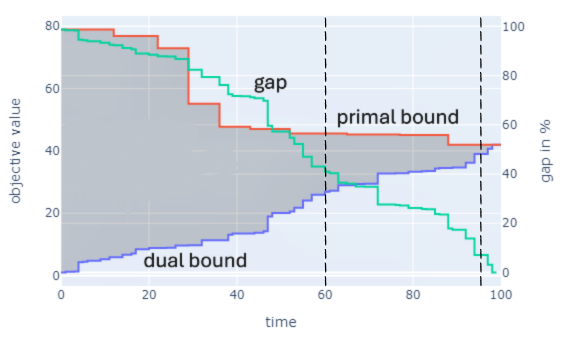
\includegraphics[width=12cm]{ejercicios/gap_gurobi_final.png} 
    \caption{evolución temporal de las cotas y el \textit{gap}. (Fuente: Gurobi)}
\end{figure}

\begin{enumerate}
    \item ¿Qué tipo de problema (\textit{maximizar o minimizar}) se está resolviendo? ¿Por qué? Es un problema de minimización porque las cotas duales son cotas inferiores (se obtienen a partir de la relajación lineal) y las primales son cotas superiores (se obtienen a partir de las soluciones enteras factibles).
    \item Indica la expresión que define el \textit{gap}. El  \textit{gap} es igual a $\frac{z^P - z^D}{z^P}$
    \item ¿Con la información disponible, qué se puede afirmar si se hubiera parado la ejecución en el $t=60$? No se puede decir que se ha obtenido la solución óptima (tiempo después se obtienen varias soluciones enteras mejores); el GAP está cerca del ~40\%. Aún hay expectativa de encontrar una solución entera mejor.
    \item ¿Con la información disponible, qué se puede afirmar si se hubiera parado la ejecución en el $t=90$? Se ha alcanzado la solución óptima pero no se puede asegurar que lo es, el GAP aún no es 0\% (o no se han cruzado las dos cotas).
\end{enumerate}


